\chapter{Direct Deep Reinforcement Learning of Decision Tree Policies}\label{sec:topin}
In this chapter, we compare deep reinforcement learning of decision tree policies (Chaper \ref{sec:intro-pomdp}) to imitation learning of decision tree policies (Sec. \ref{sec:imit}) for the CartPole MDP~\cite{cartpole}.

In particular, we attempt to reproduce the results from~\cite[Table 1]{topin2021iterative} in which authors constraint the solution space of decision tree policies to depth-2 trees.
In the original results, authors find that deep reinforcement learning to solve the interpretable rl objective (\ref{def:irl}) and Dagger or VIPER (Sec. \ref{sec:imit}) to solve the imitation learning objective (\ref{def:il}) find similar decision trees.
We find that imitation learning, despite not directly optimizing the RL objective (\ref{def:mdp-obj}) for CartPole, outperforms deep RL that optimizes (\ref{def:irl}) even though the deep RL approach directly optimizes the RL objective for CartPole (up to some trade-off with interpretability).
\section{Reproducing ``Iterative Bounding MDPs: Learning Interpretable Policies via Non-Interpretable Methods''}

\subsection{IBMDP formulation}
Given a a factored base MDP $\mathcal{M}\langle S, A, R, T, T_0\rangle$ (\ref{def:fmdp}), in order to define an IBMDP $\mathcal{M}_{IB}\langle S\times O, A\cup A_{\info}, (R, \zeta),( T, T_0, T_{info})\rangle$ (\ref{def:ibmdp}), the user needs to provide the set of information gathering actions $A_{info}$ and the reward $\zeta$ for taking those.
Authors of~\cite{topin2021iterative} propose to parametrize the set of IGAs with $i \times p$ actions $\langle v_k, i \rangle$ with $v_k$ depending on the current observation $\boldsymbol{o}_t=(L'_1, U'_1, \dots, L'_i, U'_i, \dots, L'_n, U'_n)$: $v_k = \frac{k(U'_i - L'_i)}{p+1}$.
This parametric IGAs space keeps the discrete IBMDP action space at a reasonable size while providing a learning algorithm with varied IGAs to try.

For example, if we define an IBMDP with $q=3$ for the grid world from Example~\ref{example:grid}, the grid world action space is augmented with six IGAs. 
At $t=0$, recall that $\boldsymbol{o}_0=(0, 2, 0, 2)$, so if an IGA is taken, e.g. $\langle v_2, 2 \rangle$, the effective IGA is $\langle v_2=\frac{k(2-0)}{3+1}, i \rangle = \langle 1, 2 \rangle$ which in turn effectively corresponds to an internal decision tree node $y \leq 1$.
If the current state $y$-feature value is $0.5$, then the next observation at $t=1$ is $\boldsymbol{o}_1=(0, 2, 0, 1)$. At $t=2$ if $a_t=\langle v_2, 2 \rangle$ again, it would be effectively $\langle v_2=\frac{k(1-0)}{3+1}, i \rangle = \langle 0.5, 2 \rangle$. 
This would give the next observation at $t=2$ $\boldsymbol{o}_2=(0, 2, 0, 0.5)$ and so on \dots. 

Furthermore, author propose to regularize the learned decision tree policy with a maximum depth parameter $D$.
Unfortunately, authors did not describe how they implemented the depth control in their work, hence we have to try different approaches to reproduce their results.

To control the tree depth during learning in the IBMDP, we can either give negative reward for taking $D$ IGAs in a row, or we could terminate the trajectory. 
The penalization approaches can break the MDP formalism because the reward function now depends on time while it should only depend on states and actions (\ref{def:mdp}).
Similarly, the termination approach requires a transition function that depends on time which also breaks the Makrov property.

We actually find that when $q+1$, the IBMDP information gathering space parameter, is a prime number, then as a direct consequence of the \textit{Chinese Reminder Theorem}, the current tree depth is directly encoded in the current observation $\boldsymbol{o}_t$. 
Hence, when $q+1$ is prime, we can control the depth through either transitions or rewards without tracking the time.

We will try various $\zeta$, various $q$, and various depth control in our experiments but first we describe the reinforcement learning algorithms used in~\cite{topin2021iterative}.

\subsection{Modified Deep Reinforcement Learning algorithms}
Authors of \cite{topin2021iterative} use two deep reinforcement learning baselines to which they apply some modifications in order to learn partially observable policies as required by proposition (\ref{def:po-policy}) and objective (\ref{def:irl}).

The first algorithm is a modified proximal policy optimization algorithm (PPO)(\cite{ppo}, Alg. \ref{alg:ppo}) that we present in Algorithm \ref{alg:mod-ppo}.
Authors modify the standard PPO and train a neural network policy $O\rightarrow A\cup A_{info}$ while the neural network value function is $S\times O\rightarrow A\cup A_{info}$.

The second deep reinforcement learning algorithm used is the deep Q-networks algorithm (DQN)(\cite{dqn}, Alg. \ref{alg:dqn}) that we present in Algorithm \ref{alg:mod-dqn}.
A similar modification is done to DQN to return a partially observable policy. The trained $Q$-function is approximated with a neural network $O\rightarrow \rightarrow \mathbb{R}^{|A\cup A_{info}|}$ rather than $S\times O\rightarrow \mathbb{R}^{|A\cup A_{info}|}$.
In this modified DQN, the temporal difference error target for the $Q$-function $O\rightarrow A\cup A_{info}$ is approximated by a neural network $S\times O\rightarrow A\cup A_{info}$ that is in turn trained by bootstrapping the temporal difference error with itself.

Those two variants of DQN and PPO have first been introduced in \cite{pinto} for robotics tasks with partially observable components, under the name ``asymmetric'' actor-critic. 
Asymmetric RL algorithms that have policy and value estimates using different information from a POMDP~\cite{POMDP,chap2} were later studied theoretically to solve POMDPs in Baisero's work~\cite{baisero-dqn,baisero-ppo}.
The connexions from Deep RL in IBMDPs for objective \ref{def:irl} is absent from \cite{topin2021iterative} and we defer their connexions to direct interpretable reinforcement learning to the next Chapter as our primary goal is to reproduce \cite{topin2021iterative} \textit{as is}.

Next, we present the precise experimental setup we use to reproduce~\cite[Table 1]{topin2021iterative} in order to study direct deep reinforcement learning of decision tree policies for the CartPole MDP.

\begin{algorithm}
    \KwData{IBMDP $\mathcal{M}_{IB}\langle S\times O, A\cup A_{\info}, (R, \zeta),( T, T_0, T_{info})\rangle$, learning rate $\alpha$, exploration rate $\epsilon$, partially observable Q-network parameters $\theta$, Q-network parameters $\phi$, replay buffer $\mathcal{B}$, update frequency $C$}
    \KwResult{Partially pbservable deterministic policy $\pi_{po}$}
    Initialize partially observable Q-network parameters $\theta$\\
    Initialize Q-network parameters $\phi$ and target network parameters $\phi^- = \phi$ \\

    Initialize replay buffer $\mathcal{B} = \emptyset$ \\
    \For{each episode}{
        Initialize state $\boldsymbol{s}_0 \sim T_0$ \\
        Initialize state $\boldsymbol{o}_0 = (L_1, U_1, \dots, L_n, U_n)$ \\

        \For{each step $t$}{
            Choose action $a_t$ using $\epsilon$-greedy: $a_t = \arg\max_a Q_\theta(\boldsymbol{o}_t,a)$ with prob. $1-\epsilon$ \\
            Take action $a_t$, observe $r_t$ \\
            Store transition $(\boldsymbol{s}_t, \boldsymbol{o}_t, a_t, r_t, \boldsymbol{s}_{t+1})$ in $\mathcal{B}$ \\
            Sample random batch $(\boldsymbol{s}_i, \boldsymbol{o}_i, a_i, r_i, \boldsymbol{s}_{i+1}) \sim \mathcal{B}$ \\
            $a' = \underset{a}{\operatorname{argmax}} Q_{\theta}(\boldsymbol{o}_i, a)$ \\
            $y_i = r_i + \gamma Q_{\phi^-}(\boldsymbol{s}_{i+1}, a')$ \Comment{// Compute target}
            $\phi \leftarrow \phi - \alpha \nabla_\phi (Q_\phi(\boldsymbol{s}_i, a_i) - y_i)^2$ \Comment{// Update Q-network}
            $\theta \leftarrow \theta - \alpha \nabla_\theta (Q_\theta(\boldsymbol{o}_i, a_i) - y_i)^2$ \Comment{// Update partially observable Q-network}

            \If{$t \bmod C = 0$}{
                $\theta^- \leftarrow \theta$ \Comment{// Update target network}
            }
            $\boldsymbol{s}_t \leftarrow \boldsymbol{s}_{t+1}$ \\
            $\boldsymbol{o}_t \leftarrow \boldsymbol{o}_{t+1}$ \\
        }
    }
    $\pi_{po}(\boldsymbol{o}) = \arg\max_a Q_\theta(\boldsymbol{o},a)$ \Comment{// Extract greedy policy}
    \caption{Modified Deep Q-Network (DQN)}\label{alg:mod-dqn}
\end{algorithm}


\begin{algorithm}
    \KwData{IBMDP $\mathcal{M}_{IB}\langle S\times O, A\cup A_{\info}, (R, \zeta),( T, T_0, T_{info})\rangle$, learning rate $\alpha$, policy parameters $\theta$, clipping parameter $\epsilon$, value function parameters $\phi$}
    \KwResult{Partially observable stochastic policy $\pi_{po_\theta}$}
    Initialize policy parameters $\theta$ and value function parameters $\phi$ \\
    \For{each episode}{
        Generate trajectory $\tau = (\boldsymbol{s}_0, \boldsymbol{o}_0, a_0, r_0, \boldsymbol{s}_1, \boldsymbol{o}_1, a_1, r_1, \ldots)$ following $\pi_\theta$ \\
        \For{each timestep $t$ in trajectory}{
            $G_t \leftarrow \sum_{k=t}^{T} \gamma^{k-t} r_k$ \Comment{// Compute return}
            $A_t \leftarrow G_t - V_\phi(\boldsymbol{s}_t)$ \Comment{// Compute advantage}
            $r_t(\theta) \leftarrow \frac{\pi_{po_\theta}(a_t|\boldsymbol{o}_t)}{\pi_{po_\theta}_{old}(a_t|\boldsymbol{o}_t)}$ \Comment{// Compute probability ratio}
            $L^{CLIP}_t \leftarrow \min(r_t(\theta) A_t, \text{clip}(r_t(\theta), 1-\epsilon, 1+\epsilon) A_t)$ \Comment{// Clipped objective}
            $\theta \leftarrow \theta + \alpha \nabla_\theta L^{CLIP}_t$ \Comment{// Policy update}
            $\phi \leftarrow \phi + \alpha \nabla_\phi (G_t - V_\phi(\boldsymbol{s}_t))^2$ \Comment{// Value function update}
        }
        $\theta_{old} \leftarrow \theta$ \Comment{// Update old policy}
    }
    \caption{Proximal Policy Optimization (PPO)}\label{alg:mod-ppo}
\end{algorithm}

\section{Experimental setup}
\subsection{(IB)MDP} 

We use the exact same MDP and associated IBMDPs for our experiments as~\cite{topin2021iterative} except mentioned otherwise.

\paragraph{MDP} The problem is to optimize (\ref{def:mdp-obj}) with a decision tree policy for the CartPole MDP~\cite{cartpole}.
At each time step a learning algorithm observes the cart position velocity and the pole angle and angular velocity, and can take action to push the cart left or right.
While the cart is roughly balanced, i.e., while the cart angle remains in some fixed range, the agent gets a positive reward.
If the cart is out of balance; the MDP transitions to an absorbing terminal state and gets 0 reward forever.
Like in~\cite{topin2021iterative}, we use the gymnasium \texttt{CartPole-v0} implementation~\cite{gymnasium} of the CartPole MDP in which trajectories are truncated after 200 timesteps making the maximum cumulative reward, i.e. the optimal value of objective \ref{def:mdp-obj}, to be 200.
The state features of the CartPole MDP are in $[-2, 2] \times [-2, 2] \times [-0.14, 0.14] \times [-1.4, 1.4]$.

\paragraph{IBMDP} Authors define the associated IBMDP with $\zeta=-0.01$ and parametric information gathering action space defined by $q=3$.
In addition we also try $\zeta=0.01$ and $q=2$.
The discount factor used by the authors is $\gamma=1$.

We potentially differ from the original paper setting in the way we handle maximum depth limiation. 
Indeed authors restrain the learning of policies to be equivalent to depth-2 trees but don't detail how they do so.
We hence try two different approaches as mentioned in the previous secion: terminating trajectories if the agent takes too much information gathering in a row or simply giving a reward of $-1$ to the agent everytime it takes an information gathering action past the depth limit.
We will also try IBMDPs where we do not limit the maximum depth for completeness.

\subsection{Baselines}
\paragraph{Modified DQN} as mentioned above, authors use the modified version of DQN from Algorithm~\ref{alg:mod-dqn}.
We use the exact same hyperparameters for modified DQN as the authors when possible. 
We use the same layers width (128) and number of hidden layers (2), the same exploration strategy ($\epsilon$-greedy with linearly decreasing value $\epsilon$ between 0.5 and 0.05 during the first 10\% of the training),
the same replay buffer size ($10^6$) and the same number of transitions to be collected randomly before doing value updates ($10^5$).
We also try to use more exploration during training (change the initial $\epsilon$ value to 0.9).
We use the same optimizer (RMSprop with hyperparameter 0.95 and learning rate $2.5 \times 10^{-4}$) to update the $Q$-networks.

Authors did not share what DQN implementation they used so we use the stable-baselines3 one~\cite{stable-baselines3}.
Authors did not share what activations they used so we try both $\operatorname{tanh}()$ and $\operatorname{relu}()$. 

\paragraph{Modified PPO} for the modified PPO algorithm (Alg.~\ref{alg:mod-ppo}), we can exactly match the authors hyperparameters since they use the open source stable-baselines3 implementation of PPO.

We match training budgets: we train modified DQN on 1 million timesteps and modified PPO on 4 million timesteps.

\paragraph{DQN and PPO} We also benchmark the standard DQN and PPO when learning IBMDP policies $\pi:S\times O\rightarrow A\cup A_{info}$ and when learning standard $\pi:S\rightarrow A$ policies directly in the CartPole MDP.

We summarize hyperparameters for the IBMDP and for the learning algorithms in Tables \ref{tab:ibmdp-params}, \ref{tab:ibmdp-rl1} and \ref{tab:ibmdp-rl2}.

\begin{table}[h]
    \centering
    \caption{IBMDP hyperparameters. We try 12 different IBMDPs. In \textcolor{green}{green} we highlight the hyperparameters from the original paper and in \textcolor{red}{red} we highlight the hyperparameter names for which author do not give information.}\label{tab:ibmdp-params}
    \begin{tabular}{ll}
    \toprule
    \textbf{Hyperparameter} & \textbf{Values}\\
    \midrule
    Discount factor $\gamma$ & \textcolor{green}{1} \\
    Information gathering actions parameter $q$ & 2, \textcolor{green}{3} \\
    Information gathering actions rewards $\zeta$ & \textcolor{green}{-0.01}, 0.01 \\
    \textcolor{red}{Depth control} & Done signal, negative reward, none \\ 
    \bottomrule
    \end{tabular}
    \end{table}

\begin{table}[h]
    \centering
    \caption{(Modified) DQN trained on $10^6$ timesteps. This gives four different instantiation of (modified) DQN. Hyperparameters not mentioned are stable-baselines3 default. In \textcolor{green}{green} we highlight the hyperparameters from the original paper and in \textcolor{red}{red} we highlight the hyperparameter names for which author do not give information.}\label{tab:ibmdp-rl1}
    \begin{tabular}{ll}
    \toprule
    \textbf{Hyperparameter} & \textbf{Values}\\
    \midrule
    Buffer size & \textcolor{green}{$10^6$} \\
    Random transitions before learning & \textcolor{green}{$10^5$} \\
    Epsilon stard & 0.9, \textcolor{green}{0.5} \\
    Epsilon end & \textcolor{green}{0.05} \\
    Exploration fraction & \textcolor{green}{0.1} \\
    Optimizer & \textcolor{green}{RMSprop ($\alpha = 0.95$)}\\
    Learning rate & \textcolor{green}{$2.5\times10^{-4}$}\\
    Networks architectures & \textcolor{green}{[128, 128]}\\
    \textcolor{red}{Networks activation} & $\operatorname{tanh()}$, $\operatorname{relu()}$\\
    \bottomrule
    \end{tabular}
    \end{table}

\begin{table}[h]
    \centering
    \caption{(Modified) PPO trained on $4\times10^6$ timesteps. This gives two different instantiation of (modified) PPO. Hyperparameters not mentioned are stable-baselines3 default. In \textcolor{green}{green} we highlight the hyperparameters from the original paper and in \textcolor{red}{red} we highlight the hyperparameter names for which author do not give information.}\label{tab:ibmdp-rl2}
    \begin{tabular}{ll}
    \toprule
    \textbf{Hyperparameter} & \textbf{Values}\\
    \midrule
    Steps between each policy gradient steps & \textcolor{green}{512} \\
    Number of minibatch for policy gradient updates & \textcolor{green}{4} \\
    Networks architectures & \textcolor{green}{[64, 64]}\\
    \textcolor{red}{Networks activations} & $\operatorname{tanh()}$, $\operatorname{relu()}$\\
    \bottomrule
    \end{tabular}
    \end{table}


\paragraph{Indirect methods} We also compare modified RL algorithm to imitation learning (Sec. \ref{sec:imit}).
To do so, we use VIPER or Dagger (Algs~\ref{alg:viper}~\cite{dagger}, \ref{alg:viper}~\cite{viper}) to imitate greedy neural network policies obtained with standard DQN learning directly on CartPole.
And we use Dagger to imitate neural network policies obtained with the standard PPO learning directly on CartPole. 

For each indirect method, we imitate the neural network experts by fitting decision trees on 10000 expert transitions using the CART (Alg.~\ref{alg:cart}~\cite{breiman1984classification}) implementation from scikit-learn~\cite{scikit-learn} with default hyperparameters and maximum depth of 2 like in ~\cite{topin2021iterative}.
    
\subsection{Metrics}
The key metric of this section is performance when controlling the CartPole, i.e, the average \textit{undiscounted} cumulative reward of a policy on 100 trajectories (objective \ref{def:mdp-obj} with $\gamma=1$).

For modified RL algorithms that learn a partially observable policy (or $Q$-function) in an IBMPD, we periodically extract the policy (or $Q$-function) and use Alg.\ref{alg:extract-tree} to extract a decision tree for the CartPole MDP. 
We then evaluate the tree on 100 independent trajectories in the MDP and report the mean undiscounted cumulative reward.

For standard RL applied to IBMDPs, since we can't deploy learned policies directly to the base MDP as the state dimensions mismatch (such policies are $S\times O\rightarrow A \cup A_{info}$ but the MDP states are in $S$), we periodically evaluate those IBMDP policies in a copy of the training IBMDP in which we fix $\zeta=0$ ensuring that the copied IBMDP undiscounted cumulative rewards only correspond to rewards from the base CartPole MDP (non-zero rewards in the IBMDP only occur when a reward from the base MDP is given, i.e. when $a_t\in A$ in the IBMDP (cf. Def.~\ref{def:ibmdp})).
Similarly, we do 100 trajectories of the extracted policies in the copied IBMDP and report the average undiscounted cumulative reward.

For RL applied directly to the base MDP we can just periodically extract the learned policies and evaluate them on 100 CartPole trajectories.

Since imitation learning baselines train offline, i.e, on a fixed dataset, their performances cannot be reported on the same axis as RL baselines.
For that reason, during the training of a standard RL baseline, we periodically extract the trained neural policy/$Q$-function that we consider as the expert to imitate.
Those experts are then imitated with VIPER or Dagger using 10 000 newly generated transitions and the fitted decision tree policies are then evaluated on 100 CartPole trajectories.
We do not report the imitation learning objective values (\ref{def:il}) during VIPER or Dagger training.
Every single combination of IBMDP and Modified RL hyperparameters is run 20 times.
For standard RL on either an IBMDP or an MDP with use the paper's original hyperparameters when they were specified, with depth control using negative rewards, $\operatorname{tanh()}$ activations, and we repeat this training 20 times. 

Next, we present our results when reproducing~\cite[Table 1]{topin2021iterative}.

\section{Results}

\subsection{How well do modified Deep RL baselines learn in IBMDPs?}

\begin{figure}
    \centering
    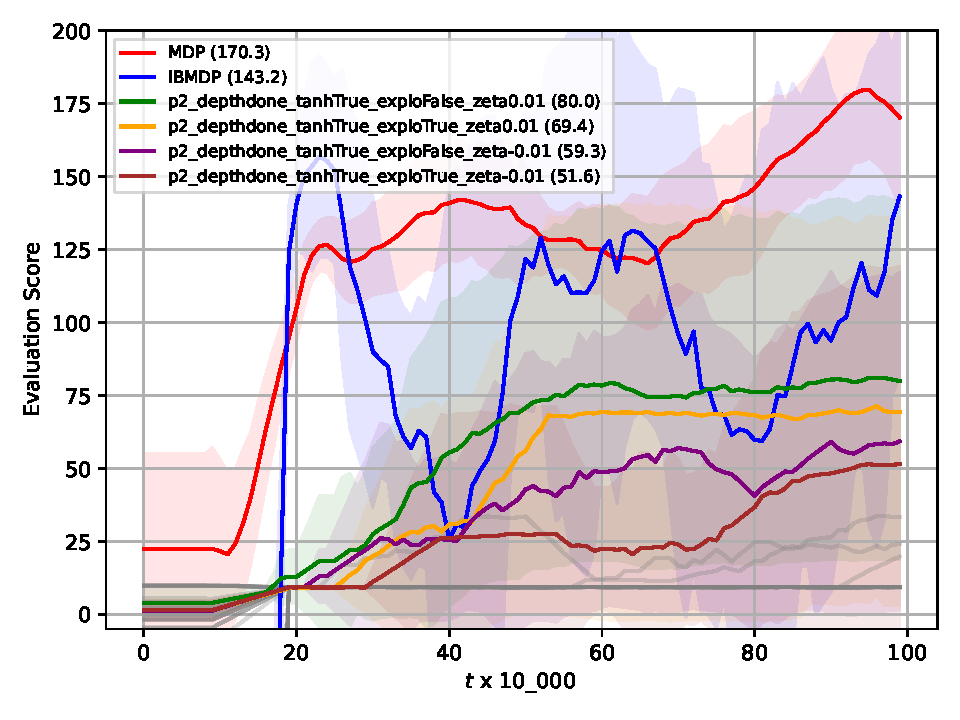
\includegraphics[width=0.7\textwidth]{images/images_part1/dqn.pdf}
    \caption{Variations of modified DQN and DQN (cf.~\ref{tab:ibmdp-rl1}), on different CartPole IBMDPs (cf. ~\ref{tab:ibmdp-params}). We give different line-styles for the learning curves for DQN applied directly on CartPole and DQN applied on the IBMDP.
    Since there are multiple possible candidates for the original paper hyperparameters, we choose to color the (modified DQN variant, IBMDP variant) pair that resulted in the best decision tree policy on CartPole among the instances that could match the original paper's.
    Shaded areas represent the confidence interval at 95\% at each measure on the y-axis.}
\end{figure}\label{fig:res-dqn}

\begin{figure}
    \centering
    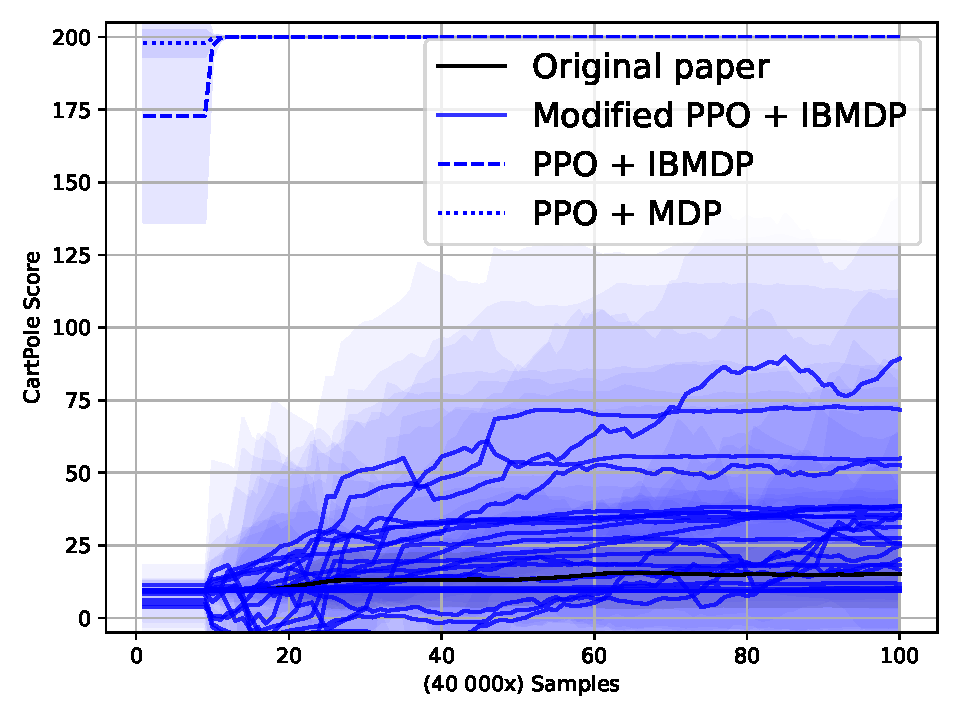
\includegraphics[width=0.7\textwidth]{images/images_part1/ppo.pdf}
    \caption{Variations of modified PPO and PPO (cf.~\ref{tab:ibmdp-rl2}), on different CartPole IBMDPs (cf. ~\ref{tab:ibmdp-params}). We give different line-styles for the learning curves for PPO applied directly on CartPole and DQN applied on the IBMDP.
    Since there are multiple possible candidates for the original paper hyperparameters, we choose to color the (modified PPO variant, IBMDP variant) pair that resulted in the best decision tree policy on CartPole among the instances that could match the original paper's.
    Shaded areas represent the confidence interval at 95\% at each measure on the y-axis.}
\end{figure}\label{fig:res-ppo}

On Figure~\ref{fig:res-dqn}, we observe that modified DQN can learn in IBMDPs--the curves have an increasing trend--but we also observe that modified DQN finds poor decision tree policies for CartPole in average--the curves flatten at the end of the x-axis and have low y-values--.
In particular, among all the learning curves that could possibly correspond to the original paper's modified DQN, the learning curve with highest final y-value is converging to decision tree policies for CartPole high poor performances.

On Figure~\ref{fig:res-ppo}, we observe that modified PPO finds decision tree policies with almost 150 cumulative rewards towards the end of training. The performance difference with modified DQN could be because we trained longer, like in the original paper.

However it could also be because DQN-like algorithm with those hyperparameters struggle to learn in CartPole (IB)MDPs.
Indeed, we notice that for DQN-like baselines, learning seems difficult in general independently of the setting.

On Figures~\ref{fig:res-dqn} and~\ref{fig:res-ppo}, we observe that standard RL baselines (RL + IBMDP and RL + MDP), learn better CartPole policies in average than their modified counterparts that learn partially observable policies (\ref{def:po-policy}). 
On Figure~\ref{fig:res-ppo}, it is clear that for the standard PPO baselines, learning is super efficient and algorithms learn optimal policies with reward 200 in few thousands steps.

In Tables ~\ref{tab:mod-dqn} and~\ref{tab:mod-ppo} we report the top-5 hyperparameters for Modified RL baselines when learning partially observable IBMDP policies in terms of extracted decision tree policies performances in CartPole control.
\begin{table}[h]
    \centering
    \caption{Top 5 Hyperparameter Configurations for modified DQN + IBMDP, bold font represent the original paper hyperparameters.}\label{tab:mod-dqn}
    \label{tab:top5_results}
    \begin{tabular}{ccccccS}
    \toprule
    Rank & $q$ & Depth control & Activation & Exploration & $\zeta$ & {Final Performance} \\
    \midrule
    1 & 3 & termination & $\operatorname{tanh}()$ & 0.9 & 0.01 & 53 \\
    2 & 2 & termination & $\operatorname{tanh}()$ & 0.5 & -0.01 & 24 \\
    \textbf{3} & \textbf{3} & \textbf{termination} & $\operatorname{tanh}()$ & \textbf{0.5} & \textbf{-0.01} & \textbf{24} \\
    4 & 2 & termination & $\operatorname{tanh}()$ & 0.5 & 0.01 & 23 \\
    5 & 2 & termination & $\operatorname{tanh}()$ & 0.9 & -0.01 & 22 \\
    \bottomrule
    \end{tabular}
    \end{table}

    \begin{table}[h]
        \centering
        \caption{Top 5 Hyperparameter Configurations for modified PPO + IBMDP, bold font represent the original paper hyperparameters.}\label{tab:mod-ppo}
        \label{tab:top5_ppo_results}
        \begin{tabular}{cccccS}
        \toprule
        Rank & $q$ & Depth Control & Activation & $\zeta$ & {Final Performance} \\
        \midrule
        1 & 3 & reward & $\operatorname{relu}()$ & 0.01 & 139 \\
        2 & 3 & done & $\operatorname{relu}()$ & 0.01 & 132 \\
        \textbf{3} & \textbf{3} & \textbf{reward} & $\operatorname{tanh}()$ & \textbf{-0.01} & \textbf{119} \\
        4 & 3 & reward & $\operatorname{relu}()$ & -0.01 & 117 \\
        5 & 3 & reward & $\operatorname{tanh}()$ & 0.01 & 116 \\
        \bottomrule
        \end{tabular}
        \end{table}


\subsection{What decision tree policies does direct reinforcement learning return for CartPole?}

\begin{figure}
    \centering
    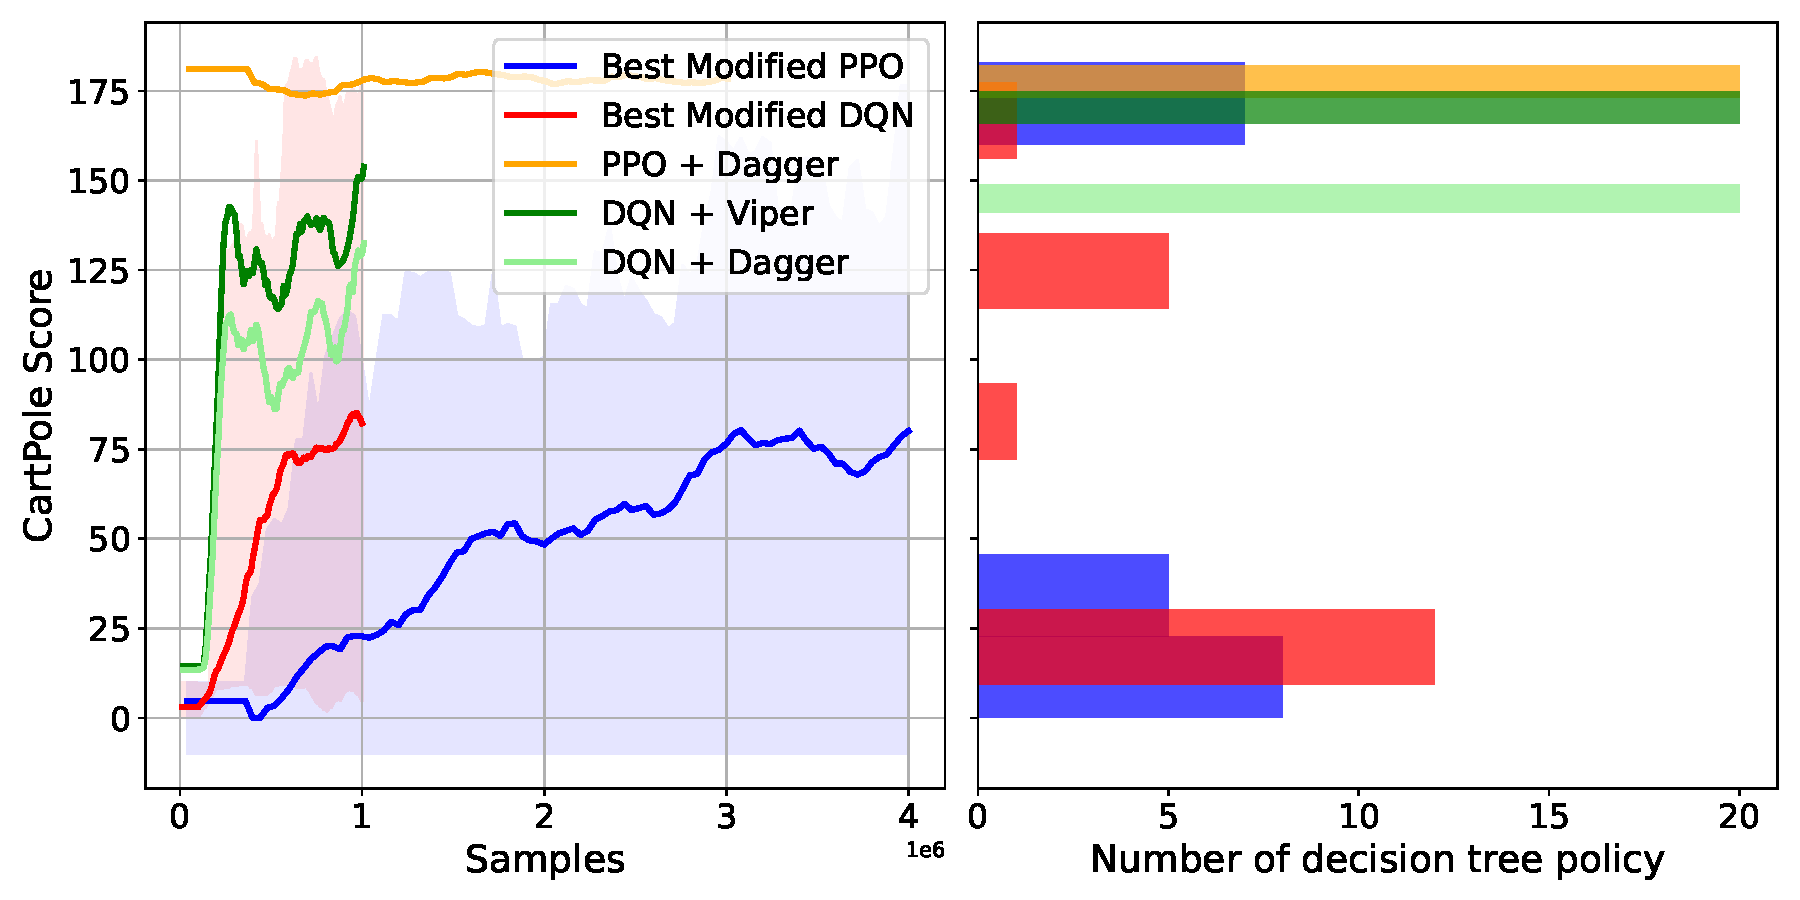
\includegraphics[width=1\textwidth]{images/images_part1/ppo_tree_study.pdf}
    \caption{(left) Mean performance of the best--w.r.t. to the RL objective (~\ref{def:mdp-obj}) for CartPole--modified RL + IBMDP combination. Shaded areas representing the min and max performance over the 20 seeds during training. (right) Corresponding scores distribution of the final decision tree policies performances w.r.t. to the RL objective (~\ref{def:mdp-obj}) for CartPole.}\label{fig:ppo-trees}
\end{figure}


\begin{figure}[htbp]
    \centering
    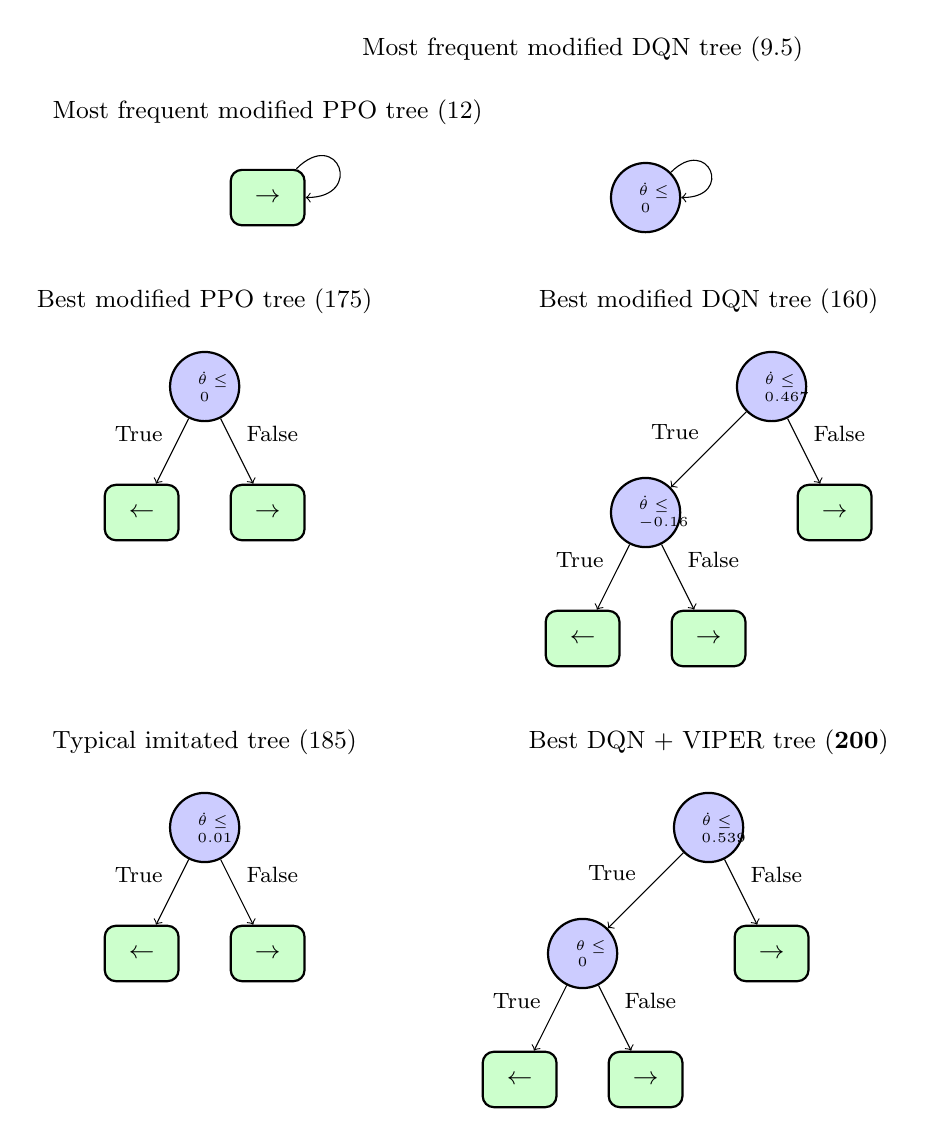
\begin{tikzpicture}[
        scale=0.8,
        decision/.style={circle, draw, thick, fill=blue!20, text width=0.5em, text centered, minimum height=2.5em, font=\tiny},
        leaf/.style={rectangle, draw, thick, fill=green!20, text width=2em, text centered, rounded corners, minimum height=2em, font=\small},
        edge_label/.style={font=\footnotesize, midway}
    ]

        \node[leaf] (tree7_root) at (-2,3) {$\rightarrow$};
        \draw[->] (tree7_root) to[out=45,in=0,looseness=5] (tree7_root);

        \node[decision] (tree7_root) at (4,3) {$\dot{\theta} \leq 0$};
        \draw[->] (tree7_root) to[out=45,in=0,looseness=5] (tree7_root);
        
        % Tree 4: if x <= 0.5 move right else move left
        \node[decision] (tree4_root) at (-3,0) { $\dot{\theta}\leq 0$};
        \node[leaf] (tree4_right) at (-4,-2) {$\leftarrow$};
        \node[leaf] (tree4_left) at (-2,-2) {$\rightarrow$};
        \draw[->] (tree4_root) -- (tree4_right) node[edge_label, above left] {True};
        \draw[->] (tree4_root) -- (tree4_left) node[edge_label, above right] {False};
        

        % Tree 7: if x <= 0.5 and y <= 0.5 move right else move down
        \node[decision] (tree7_root) at (6,0) {$\dot{\theta}\leq 0.467$};
        \node[decision] (tree7_y) at (4,-2) {$\dot{\theta}\leq -0.16$};
        \node[leaf] (tree7_right) at (3,-4) {$\leftarrow$};
        \node[leaf] (tree7_down) at (5,-4) {$\rightarrow$};
        \node[leaf] (tree7_down2) at (7,-2) {$\rightarrow$};
        \draw[->] (tree7_root) -- (tree7_y) node[edge_label, above left] {True};
        \draw[->] (tree7_root) -- (tree7_down2) node[edge_label, above right] {False};
        \draw[->] (tree7_y) -- (tree7_right) node[edge_label, above left] {True};
        \draw[->] (tree7_y) -- (tree7_down) node[edge_label, above right] {False};




        % Tree 4: if x <= 0.5 move right else move left (Second row, left)
        \node[decision] (tree4_root2) at (-3,-7) { $\dot{\theta}\leq 0.01$};
        \node[leaf] (tree4_right2) at (-4,-9) {$\leftarrow$};
        \node[leaf] (tree4_left2) at (-2,-9) {$\rightarrow$};
        \draw[->] (tree4_root2) -- (tree4_right2) node[edge_label, above left] {True};
        \draw[->] (tree4_root2) -- (tree4_left2) node[edge_label, above right] {False};


        % Tree 7: if x <= 0.5 and y <= 0.5 move right else move down (Second row, right)
        \node[decision] (tree7_root2) at (5,-7) {$\dot{\theta}\leq 0.539$};
        \node[decision] (tree7_y2) at (3,-9) {$\theta\leq 0$};
        \node[leaf] (tree7_right2) at (2,-11) {$\leftarrow$};
        \node[leaf] (tree7_down3) at (4,-11) {$\rightarrow$};
        \node[leaf] (tree7_down4) at (6,-9) {$\rightarrow$};
        \draw[->] (tree7_root2) -- (tree7_y2) node[edge_label, above left] {True};
        \draw[->] (tree7_root2) -- (tree7_down4) node[edge_label, above right] {False};
        \draw[->] (tree7_y2) -- (tree7_right2) node[edge_label, above left] {True};
        \draw[->] (tree7_y2) -- (tree7_down3) node[edge_label, above right] {False};
        

        % Labels
        \node[above] at (-2,4) {{\small Most frequent modified PPO tree (12)}};
        \node[above] at (3,5) {{\small Most frequent modified DQN tree (9.5)}};

        \node[above] at (-3,1) {{\small Best modified PPO tree (175)}};
        \node[above] at (5,1) {{\small Best modified DQN tree (160)}};
        \node[above] at (-3,-6) {{\small Typical imitated tree (185)}};
        \node[above] at (5,-6) {{\small Best DQN + VIPER tree (\textbf{200})}};


    \end{tikzpicture}
    \caption{Trees obtained by Deep RL in IBMDPs against trees obtained with imitation (CartPole cumulative rewards). $\theta$ and $\dot{\theta}$ are respectively the angle and the angular velocity of the pole}
    \label{fig:trees-drl}
\end{figure}


On Figure~\ref{fig:ppo-trees}, we isolate the best performing algorithms instantiations that learn decision tree policies for CartPole.
We compare the best modified DQN or modified PPO to imitation learning baselines that use the surrogate imitation objective (~\ref{def:il}) to find CartPole decision tree policies.
We find that despite having poor performances in \textit{average}, the modified deep reinforcement learning baselines can find very good decision tree policies as shown by the min-max shaded areas on the left of Figure~\ref{fig:ppo-trees} and the corresponding estimated density of final trees performances.
However this is not desirable, a user typically wants an algorithm that can consistently find good decision tree policies.
As shown by the estimated densities, indirect methods consistently find good decision tree policies (the higher modes of distributions are on the right of the plot).
On the other hand, the final trees returned by direct RL methods seem equally distributed on both extremes of the scores.

On Figure~\ref{fig:trees-drl}, we present the best decision tree policies for CartPole returned by modified DQN and modified PPO.
We used Algorithm~\ref{alg:extract-tree} to extract 20 trees from the 20 partially observable policies returned by the modified deep reinforcement learning algorithms over the 20 training seeds.
We then plot the best tree for each baseline.
Those trees get an average reward of roughly 175.
Similarly, we plot a representative tree for imitation learning baseline as well as a tree that is optimal for CartPole w.r.t. (~\ref{def:mdp-obj}) obtained with VIPER. 
Unlike for direct methods, the trees returned by imitation learning are extremely similar across seeds. In particular they often only vary in the scalar value used in the root node but in general have the same structure and test the angular velocity.
On the other hand the most frequent trees across seeds returned by modified RL baselines are ``trivial'' decision tree policy that either repeat the same base action forever or repeat the same IGA (Def. ~\ref{def:ibmdp}) forever.


\section{Discussion}
We have shown that compared to learning non-interpretable neural network policies for the base MDP or some associated IBMDP, reinforcement learning of partially observable policies in IBMDP is less efficient (cf. Figures~\ref{fig:res-dqn} and~\ref{fig:res-ppo}). 
As a consequence, only a handful of modified RL runs are able to learn decision tree policies that are on par with imitated trees (cf. Figure~\ref{fig:ppo-trees}).

In the next chapter, we highlight the connections between direct interpretable RL (Def.~\ref{def:irl}) and POMDPs to get insights on the hardness of direct reinforcement learning of decision trees.